
\chapter{Introduction}


%\subsection*{super-short-intro, inizia con lo scopo del lavoro è solo cosa è stato fatto}

This work aims to investigate the possibility of estimating a patient's respiratory rate using a sensor pressure mattress and how a rocking bed could influence its use. 
At first, it is focused on studying approaches to extract the breath and heart rate from pressure sensors using a dataset already available from previous studies. 
Then the work is focused on respiratory rate, and for this reason, it is conducted data collection using an innovative pressure textile-sensor mattress and a cardiorespiratory as ground truth: the primary objective is to collect data to understand the feasibility of extracting breath rate from the mat in case of stationary bed; the second goal is to understand if the movement of the rocking bed could influence the signal. 
In the second part, a pipeline to analyse the extracted data is created: from each mattress sensor, the signals are processed to exclude the ones without meaningful information and designed metrics that asset the confidence that from a sensor could be extracted a respiratory pattern. The remains signals are filtered to eliminate noise using multiresolution analysis of the maximal overlap discrete wavelet transform and Savitz-Golay filter to obtain a clean wave from which could be counted the number of breaths a person in a minute. As a result, the respiration rate per minute of the person is obtained and compared with the cardiopulmonary polysomnography to asset the error. The influence of the rocking bed on the mattress is obtained via the comparison of the mattress performance on the stationary bed. As a result of the pipeline is also available a heat-map to visualise where these best channels are positioned in respect of the body and so in the mattress.


\newpage


\subsubsection{Parte succosa}
Sleep is one of the most important physiological functions. Sleep quality can affect physical and mental wellness; for this reason, it is crucial to monitor vital signs and sleep stages without interfering with natural sleep. 
The state-of-the-art to monitor physiological data during sleep is polysomnography \cite{Penzel2016ModulationsPolysomnography}, which involves recording sleep stages, respiratory rate, heart and other parameters. However, this procedure is time-consuming, complicated, expensive,
 invasive for the patient and only sometimes available in hospitals. Even in its simplified version, cardiorespiratory polysomnography \cite{CallejaComparisonApnoea}, where are involved just nose cannulas, chest belts and electrodes for an electrocardiogram (ECG) and does not track neurophysiological variables, the patient is subjected to physical discomfort throughout the night.

Breathing monitoring is also crucial because the population present a higher percentage of 
sleep-related breathing disorders that can be studied and monitored with this instrument, like sleep apnoea/hypopnoea syndrome (SAS) \cite{SasPatients}, 
where the individuals experience a collapse 
of the airway in deeper sleep states. The ability to monitor it allows for a faster and closer intervention in severe cases. 

Also, in the study of sleep stages \cite{Gasmi2020SleepVariables}, it is known that different muscle tones, brain wave patterns, eye movements and heart and breathing rate alterations characterise every phase and stage.
So if focused on one of the vital signs that characterise the different sleep stages, like respiratory rate, which in particular slowly becomes more stable in the Non-Rapid Eye Movement (NREM) phase and increases during the Rapid Eye Movement (REM) phase, this characterisation of the different stages gives the possibility to understand in which stage a person is based just on the respiratory signal\cite{Pal2022BreathingWakefulness}.

Nowadays, it is possible to achieve this goal using different unobtrusive methods, such as radar technology \cite{RadarSensor}. The limitation of this approach lies in the fact that in case of the presence of another person in the room, in a hospital condition like a nurse or doctor, or even from fans or oxygen concentrators, could be a source of noise for the radar that could lead to incorrect prediction. It can also be disturbed by the movement of the patient itself \cite{LauteslagerValidation}. Another possibility is to use video cameras with infrared filters \cite{CamerasBasedVitalSigns}; even if this approach seems promising, it leads to personal privacy concerns. 

On the market are also available smartwatches, like Garmin \cite{garminUrl}, that can estimate multiple vital signs with good precision \cite{GarminArticol}, but are devices that need to be worn all night that for some people could lead to discomfort, in case the batteries run out we lost the tracking and mostly does not give the possibility to extract the raw data. It is also possible to find under-mattress ballistocardiography-based sensors\cite{Tenhunen2013EmfitBreathing}, like Emfit \cite{emfitUrl}, that in case of multiple people inside the bed need to be placed in half of it and the wrong position can lead to inaccurate measurement.

In this thesis, it is decided to use unobtrusive methods not to cause discomfort to the user, which could also give us the possibility to track vital signs. 
However, the decision of which type of method it is also led from the availability, in the lab where this thesis is carried out, of a rocking bed part of the \textit{Somnomat}\cite{DevelopingSleep} project. This rocking bed aims to interact with the person and study how to improve sleep quality via vestibular stimulation. Also, in this case, the possibility of tracking vital signs could be significant, so the possibility of integrating unobtrusive methods with the Somnomat is part of this thesis.
For all this reason, the choice fell to pressure sensor mattresses.
They can be installed over the standard mattress and are now available as textile-sensor, which means that they can be as thin as possible and lead to less possible discomfort, but at the same time, can be used to track the respiratory rate and, depending on area density and sampling frequency, even hearth rate. 

Inside the project, it is first used pressure-sensor textiles mattresses from \textit{Sensomative} \cite{sensomativeUrl} has 14 x 28 sensor elements for a total sensor area of 40cm x 80cm that can cover the width of a regular bed, visible in \ref{fig:sensomativeBed},with a sampling rate of 50Hz. Due to the small area needing to be positioned in a specific position and case, the patient moves; it is possible not to have any more information. Previous studies have brought out the possibility of estimating breathing patterns and heart rates; since the data from this mattress and the ground truth data from polysomnography are available, both possibilities are explored.

\begin{figure}[h]
    \centering
    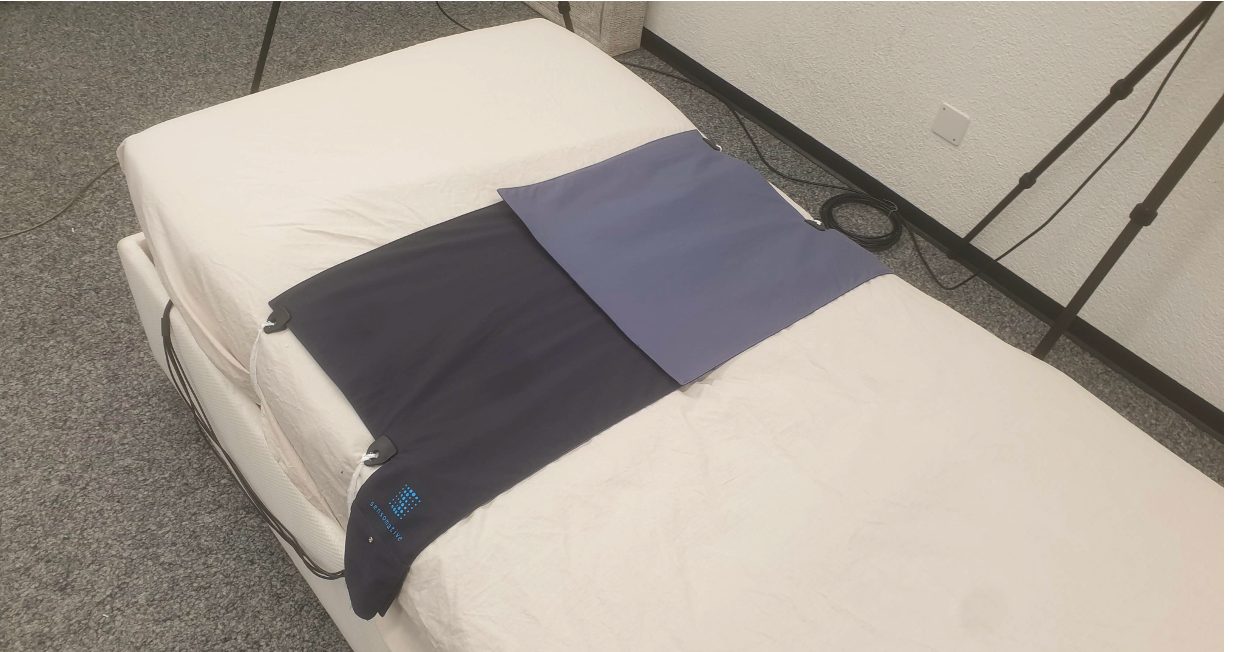
\includegraphics[width=0.5\textwidth]{img/sensomative.png}
    \caption{Sensomative over a bed}
    \label{fig:sensomativeBed}
\end{figure}

After evaluating a possible valid approach to this data, we decide to use it on a second mattress, from \textit{SensingTex} \cite{SensingConnectivity} that is already installed in a hospital ward of the \textit{University of Bern} for the study research on movement disorders during sleep in patients with Parkinson’s disease. Therefore the ability to estimate breath and heart rate could be helpful in this study.
This mattress has a lower sampling frequency (10Hz) and 22 x 40 sensor elements for a total area of 94cm x 192cm that can cover a standard bed area.


\begin{figure}[h]
    \centering
    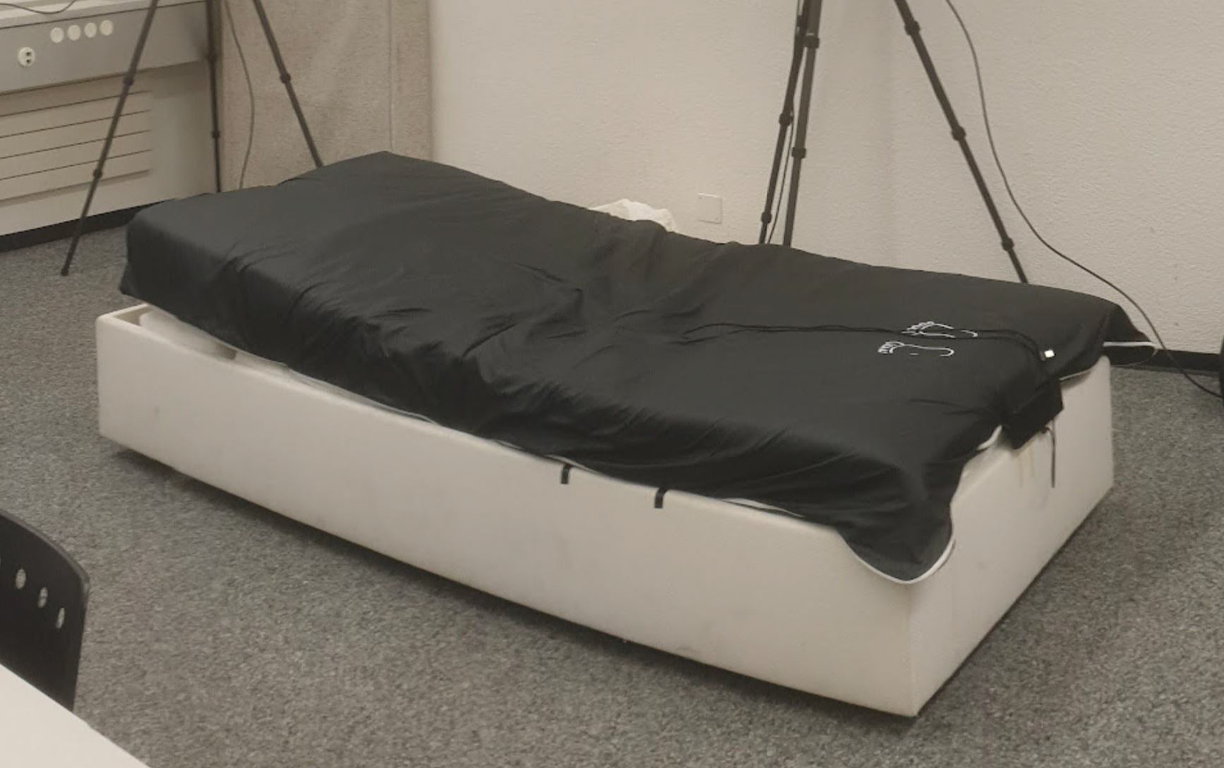
\includegraphics[width=0.5\textwidth]{img/sensingtex.png}
    \caption{Sensomative over a bed}
    \label{fig:sensingtex}
\end{figure}


Raw data extracted from the mattress can be viewed together to visually see the position and the person's movement on it; it appears as a heatmap: since pressure sensors could record the different pressures exerted by the presence/absence of a body on it or by its parts. 
%insert part image to make understand 
So it is possible to create a heat map to show the variation in colour of the intensity of the pressure, which can produce the shape of a person on the mattress.


\begin{figure}[h]
    \centering
    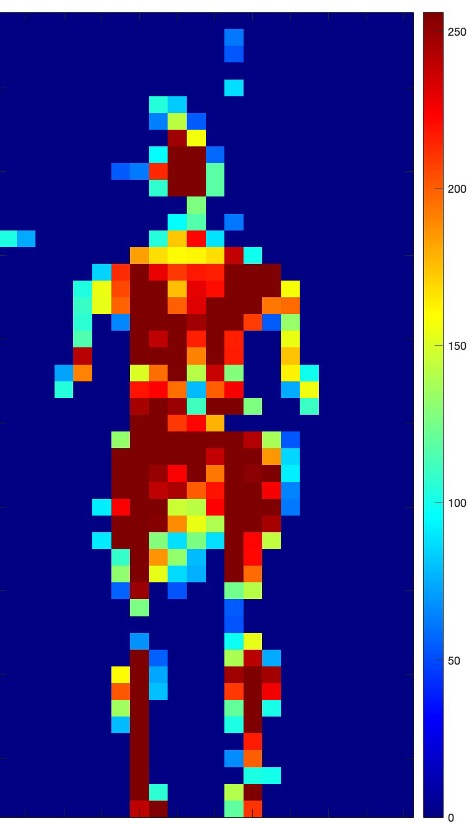
\includegraphics[width=0.5\textwidth]{img/sensingtex_2.jpg}
    \caption{Sensomative over a bed}
    \label{fig:sensingtexData}
\end{figure}


Looking closer into signals of singles channels is possible to see a pattern that resembles a breathing rhythm, similar to the data that can be retrieved from the nasal pressure exerted on the cannula of cardiorespiratory polysomnography.
This pattern was the key factor in deciding to use this sensor mattress (hereafter referred to as ``sensor mat'' or ``mat"). 

Since the data on the rocking bed were not collected before, it is necessary to conduct a data collection with two main objectives:
The primary is to collect data to understand the feasibility of extracting breath rate from the mat; the second goal is to understand if the movement of the rocking bed could influence the signal.
The participants are six, half male and half female, between 20 and 30 years old.
Each participant wears a cardiorespiratory wireless and portable polysomnography device (Nox A1 PSG of Nox Medical\cite{WirelessSystem}) that monitors nasal pressure, pulse, and heart rate with ECG and respiratory inductance plethysmography (RIP), which is a method of evaluating pulmonary ventilation by measuring the movement of the chest and abdominal wall. 


The protocol is divided into two phases:

The setting for the first phase involves the pressure mat over a standard bed. During the night and through the different sleep stages, the breath rate increase or decreases, so we decide to insert a similar variability in our data. We asked the participant to perform a set of five jumps and then lie down in a specific position for four minutes. After this period, they had to stand up, repeat the five jumps and lied down again. The total position performed is four with the following pattern: supine, left side, prone, right side and with a total of twenty jumps.


The setting for the second phase, since in this part we want to collect the data while the Somnomat is moving, we fixed the period for the movement of the bed at 4 seconds (15 periods in a minute) with an acceleration of 0.25 $m/s^2$. Also, for this phase, they have been asked to turn around following the specific pattern: supine, left side, prone, right side and remain in that position for 4 minutes.

This results in a recording of 32 minutes long for each participant divided into 4 minutes in each of the four positions with a standard bed and with Somnomat.


SensingTex total number of sensors is 1056, but they are never all significant at the same time. A person's body can not cover the entire mattress and activate all the sensors (hereafter referred to as ``Channels") simultaneously. Consequently, this leads to the necessity of an algorithm to discriminate the ones from whom it is possible to extract valuable information.
Many of these channels are stationary on a value; others present just interference from the mattress. It is possible to retrieve a respiratory pattern from just a few sensors and then extract the respiratory rate per minute (rpm). Therefore becomes necessary to design a metric that underlines these channels. 
This metric must be interpreted as confidence expressed in percentual of the goodness of the signal; at the same time is necessary to have a workflow that, from mattress data, could estimate a person's respiratory rate. This led to the creation of a pipeline that estimates the rpm based on the previous minute. Since the data collected are not in real-time because they come from the data collection, the real-time replicate with a moving window of 60 seconds long that moves on the data with an interval of 10 seconds.




$ c\longrightarrow$ 

At the same time is necessary to have a workflow that from mattress data could estimate a person's respiratory rate, this led to the creation of a pipeline that estimates the rpm based on the previous minute. Since the data collected are not in real-time because they come from the data collection the real-time replicate with a moving window with an interval of 10 seconds for each window.


$ x\longrightarrow$ 





DUBBIO SUL FATTO CHE SIA FATTO IN SEMI-REALTIME

\subsection*{citazioni, cosa è stato fatto con contesto e citazioni}


 % \cite{Bakker2021EstimatingSeverity}. 
%Respiration is also central in 
% one of the most common sleep disorders, sleep apnea, in this case, causes them to experience reduced time in stage N3 and REM sleep. si può every da 



\subsection*{indice in forma discorsiva \\ lo compilo come ultime cosa}

\subsection*{Acknowledgement}
The project is carried out in collaboration with \textit{Sensory-Motor System Lab} of Prof.~Robert Riener at \textit{Eidgenössische Technische Hochschule 
(ETH) Zürich} and supervised by Dr.~Alexander Breuss, Dr.~Oriella Gnarra and Dr.~Manuel Fujis.



\begin{comment}

\newpage
\begin{enumerate}
    \item  \textbf{Introduzione} \\  strutturato in 3 parti: 0.5 a 1 pagina di super-short-intro,descrive cosa è stato fatto dando anche il contesto (con citazioni) e riassunto di cosa ci sarà nei capitoli
    \item \textbf{Preliminaries} \\ contiene al suo interno tutta la parte di stato dell'arte dei seguenti argomenti e tutte le informaizoni necessarie per comprendere la tesi.
    \begin{enumerate}
        \item \textbf{Sleep Stages} \\ Il progetto nasce nel contesto di avere la necessita di poter monitorare la respirazione dei pazienti durante la notte, dalla letteratura si evince come la variazione nella respirazione possa essere usato per tracciarli.
        \item \textbf{Respiratory Rate} \\ Parlando di repirazione durante la tesi è necessario introdurre come funzioni la respirazione e come si definisca un respiro.
        \item \textbf{Cariorespiratory Polysomnography} \\ Come si effettuano ad oggi i montoraggi delle respirazione in ospedale, evidenzaindone i limiti.
        \item \textbf{Unobstrusive approaches} \\ citazione di altri sistemi usati ora, non ustrusivi e i motivi per cui non si vogliano usare nel nostro caso
        \item \textbf{Pressure Sensor Mattress} \\ stato ell'arte di cosa si possa fare con i materassi a pressione e similari
    \end{enumerate}
    \item \textbf{Methods} 
    \begin{enumerate}
        \item \textbf{Instrument} \\ strumenti coinvolti nella tesi
        \begin{enumerate}
            \item \textbf{SensingTex} \\ materasso grande brutto 10hz
            \item  \textbf{polisomnografia NOXA1} \\ utilizzata per tracciare la respirazione del soggeto
            \item \textbf{Somnomat} \\ letto che si muove, si vuole capire se sia utilizzabile insieme al materasso
        \end{enumerate}  
        \item  \textbf{Data Collection} \\ descrizione della necessità di avere dati per poter studiare la possibilitò di estrarre il ritmo respiratorio
        \begin{enumerate}
            \item \textbf{Normal Bed} \\ letto normale, le persone fanno 4 salti e poi si sdraiano in 4 posizioni diverse (totale 16 salti). serve per avere variabilità nei dati
            \item  \textbf{rocking bed, somnomat } \\ letto che si muove, persona sdraiata sopra che si gira in 4 posizioni, serve per vedere possibili alterazioni nei dati dovute dal movimento del letto
        \end{enumerate}  
    \end{enumerate}  
    \item  \textbf{Data Analysis} \\ Descrizione della pipeline, dai dati del materasso, preprocessamento, filtri vari, al numero di respiri al minuto per quel specifico minuto.
    \begin{enumerate}
        \item \textbf{Weighted and binary} \\ la pipeline viene creata sia dando un peso ai vari controlli effettuati sul segnale, sia rendendoli binari (o passa o non passa)
        \item  \textbf{Pipeline} \\ Descrizione effettiva della pipeline
        \begin{enumerate}
            \item \textbf{Excluding criteria} \\ criteri di esclusione dei canali, non si effettuano ulteriori analisi.
            \item  \textbf{SNR ratio} \\ deve rimanere in un intervallo, però avevo fatto casino inserendolo quindi non so se voglio citarlo
            \item  \textbf{Wavelet} 
            \begin{enumerate}
                \item teoria di come funziona
                \item applicazione nel progetto
            \end{enumerate} 
            \item \textbf{Savitz-Golay filter}
            \begin{enumerate}
                \item teoria di come funziona
                \item applicazione nel progetto
            \end{enumerate} 
            \item \textbf{Subsequent analyses of the filtered signa} \\ analisi sul segnale filtrato, controllo del numero di respiri, controllo della distanza tra picchi e valli che viene intesa sia come durata (distanza sull'asse del tempo in un intervallo +-20\%) oppure distanza euclidea picco valle (sempre +- 20\%).
        \end{enumerate} 
        \item \textbf{Result of the Pipeline (visual)} \\ risultati visuali ottenuti dalla pipeline. quidni la possibilità di visualizzare dove son i canali migliori e farci delle considerazioni.
    \end{enumerate} 
    \item \textbf{Result}
    \begin{enumerate}
        \item \textbf{Evaluation Metrics} \\spiegazione delle metriche utilizzate e la motivazione
        \begin{enumerate}
            \item Mean absolute error (MAE)
            \item Mean absolute percentage error (MAPE)
            \item Root Mean Square Error (RMSE)
        \end{enumerate} 
        \item \textbf{Result for Wavelet}
        \begin{enumerate}
            \item Bland-Altman plot 77durante la discussione su mi hanno detto che è meglio utilizzare questi per raprpesentare i risultati. ma avendo pochi dati non saprei
        \end{enumerate} 
        \item \textbf{Result for sg filter}
        \begin{enumerate}
            \item Bland-Altman plot
        \end{enumerate} 
        \item \textbf{Comparison between the two approaches (wavelet and SG filter)} \\ piccolo commento su una che va meglio dell'altro, sg filter >> wavelet
        \item  \textbf{Discussion performance on normal vs rocking bed)} \\ spiegre che funziona comnque a prescindere
    \end{enumerate} 
    \item \textbf{Conclusion and future discussin} \\ gli ampliamenti futuri ed un sunto sul fatto che si possa usare
\end{enumerate}
\end{comment}